\documentclass[]{article}
\usepackage{graphicx}
\usepackage{amsmath,amssymb,amsthm}
\usepackage{empheq}
\usepackage{float}
\usepackage[left=0.85in,top=0.85in,right=0.85in,bottom=0.85in]{geometry} % Document margins

% Title Page
\title{CS 6640 Project 4}
\author{Travis Allen, u1056595}


\begin{document}
	\maketitle
	
	\newpage
	\tableofcontents
	\newpage
	\section{Preliminaries}

	\vskip 10pt

	\textbf{I chose to do project 4a: Image Mosaicing.} The code for this project can be found in the \texttt{proj\_4.py} and \texttt{functions.py} files. \texttt{proj\_4.py} contains the actual algorithm developed to make a mosaic of greyscale images whose correspondences are documented in a \texttt{.json} file. \texttt{functions.py} contains some useful functions that would have otherwise crowded the \texttt{proj\_4.py} file. My solution to this project relies on \texttt{numba} for some parts, so you must have that installed to run my code. I use it because it dramatically speeds up the run time of the feathering algorithm. I have also included \texttt{.json} files for the images shown in this report, as well as the images themselves. 

\section{Methods}
	To build the mosaics, I set up a system of equations as follows:
	
	\[\left(\begin{array}{cccccccc}
		-x_{1} & -y_{1} & -1 & 0 & 0 & 0 & x_{1} x_{1}^{\prime} & y_{1} x_{1}^{\prime} \\
		-x_{2} & -y_{2} & -1 & 0 & 0 & 0 & x_{2} x_{2}^{\prime} & y_{2} x_{2}^{\prime} \\
		&&&\vdots&&&&\\
		-x_{N} & -y_{N} & -1 & 0 & 0 & 0 & x_{N} x_{N}^{\prime} & y_{N} x_{N}^{\prime} \\
		0 & 0 & 0 & -x_{1} & -y_{1} & -1 & x_{1} y_{1}^{\prime} & y_{1} y_{1}^{\prime} \\
		0 & 0 & 0 & -x_{2} & -y_{2} & -1 & x_{2} y_{2}^{\prime} & y_{2} y_{2}^{\prime} \\
		&&&\vdots&&&&\\
		0 & 0 & 0 & -x_{N} & -y_{N} & -1 & x_{N} y_{N}^{\prime} & y_{N} y_{N}^{\prime}
	\end{array}\right)\left(\begin{array}{c}
		p_{11} \\
		p_{12} \\
		p_{13} \\
		p_{21} \\
		p_{23} \\
		p_{23} \\
		p_{31} \\
		p_{32}
	\end{array}\right) = \left(\begin{array}{c}
		-x_{1}^{\prime} \\
		-x_{2}^{\prime} \\
		\vdots \\
		-x_{N}^{\prime} \\
		-y_{1}^{\prime} \\
		-y_{2}^{\prime} \\
		\vdots \\
		-y_{N}^{\prime}
		\end{array}\right)\]
Where each $(x_i,y_i)$ is a known correspondence point in the base image and each $(x'_i,y'_i)$ is a known correspondence point in the image to be transformed, and each $p_{ij}$ is unknown. The building of this equation occurs in \texttt{proj\_4.py} lines \texttt{97-119}. Then, I solve this system with the singular value decomposition. This process is performed in the \texttt{svd\_solve()} function in \texttt{functions.py} lines \texttt{7-25}. This gives the coefficients $p_{i,j}$ to form the following transformation matrix:
\[\left(\begin{array}{ccc}
	p_{11} & p_{12} & p_{13} \\
	p_{21} & p_{23} & p_{23} \\
	p_{31} & p_{32} & 1
\end{array}\right)\]

Each homogeneous coordinate in the image is multiplied by this transformation. The result is a non-homogeneous coordinate, so it is normalized by the third coordinate in each coordinate vector so that the resulting coordinates are homogeneous. The result of this process is the locations of each intensity with regards to the base image (non-primed coordinates in the above equation). This is implemented in the \texttt{transform()} function in \texttt{functions.py} lines \texttt{28-56}. 

At this point, I am able to use these tools to build mosaics of perspectively equivalent images with known correspondence points. I heard some talk among other students in the class that a way to improve the quality of the mosaic is to introduce some interpolation to fill in the black lines created in the mosaics shown in later parts of this report. I interpret these lines as the ``contours" of the warp, and they are produced because after both the multiplication of each coordinate by the transformation matrix, and the normalization of each coordinate to a homogeneous coordinate, the result is a floating point number and not an integer. Because array indices must be integers, a decision must be made here about how to treat these floating point indices. I tried using the \texttt{numpy.ceil()}, \texttt{numpy.floor()}, and \texttt{numpy.round()} functions, and found the results to be very similar, so much that they were indistinguishable to a casual observer. In all cases, these methods leave black lines that are visible on the image. \textbf{There was no mention of a need to implement a more sophisticated interpolation method than these in the project instructions, so I haven't done that.} However, I recognize that it would likely add to the quality of the mosaic, so I've described my hypothetical procedure for implementing interpolation below.

If I had more time to complete this project, I would implement the following scheme for interpolation. First I would take the untransformed image and apply the transformation matrix $P$ to each of its coordinates, and then normalize them in exact accordance with the procedure described above. Then, I would determine the smallest integer bounding box of this transformed image (essentially the shadow of the transformed image) and transform the coordinates that fit inside that box with the inverse transformation matrix, $P^{-1}$. The result of this process are ``new" floating point coordinates. It seems to me (informed by my limited foray into this method) that determining the bounding box and the pixels that sit inside it is the crux of this method. Then, I would take the original integer coordinates of the untransformed image and use those and their associated intensities to create a 2D interpolation function with \texttt{scipy.interpolate.interp2d()}. I would then use this 2D interpolation function to map the ``new" floating point coordinates to their respective locations on the canvas. This process is shown in the following diagram for a marginal increase in clarity. 

\begin{figure}[H]
	\centering
	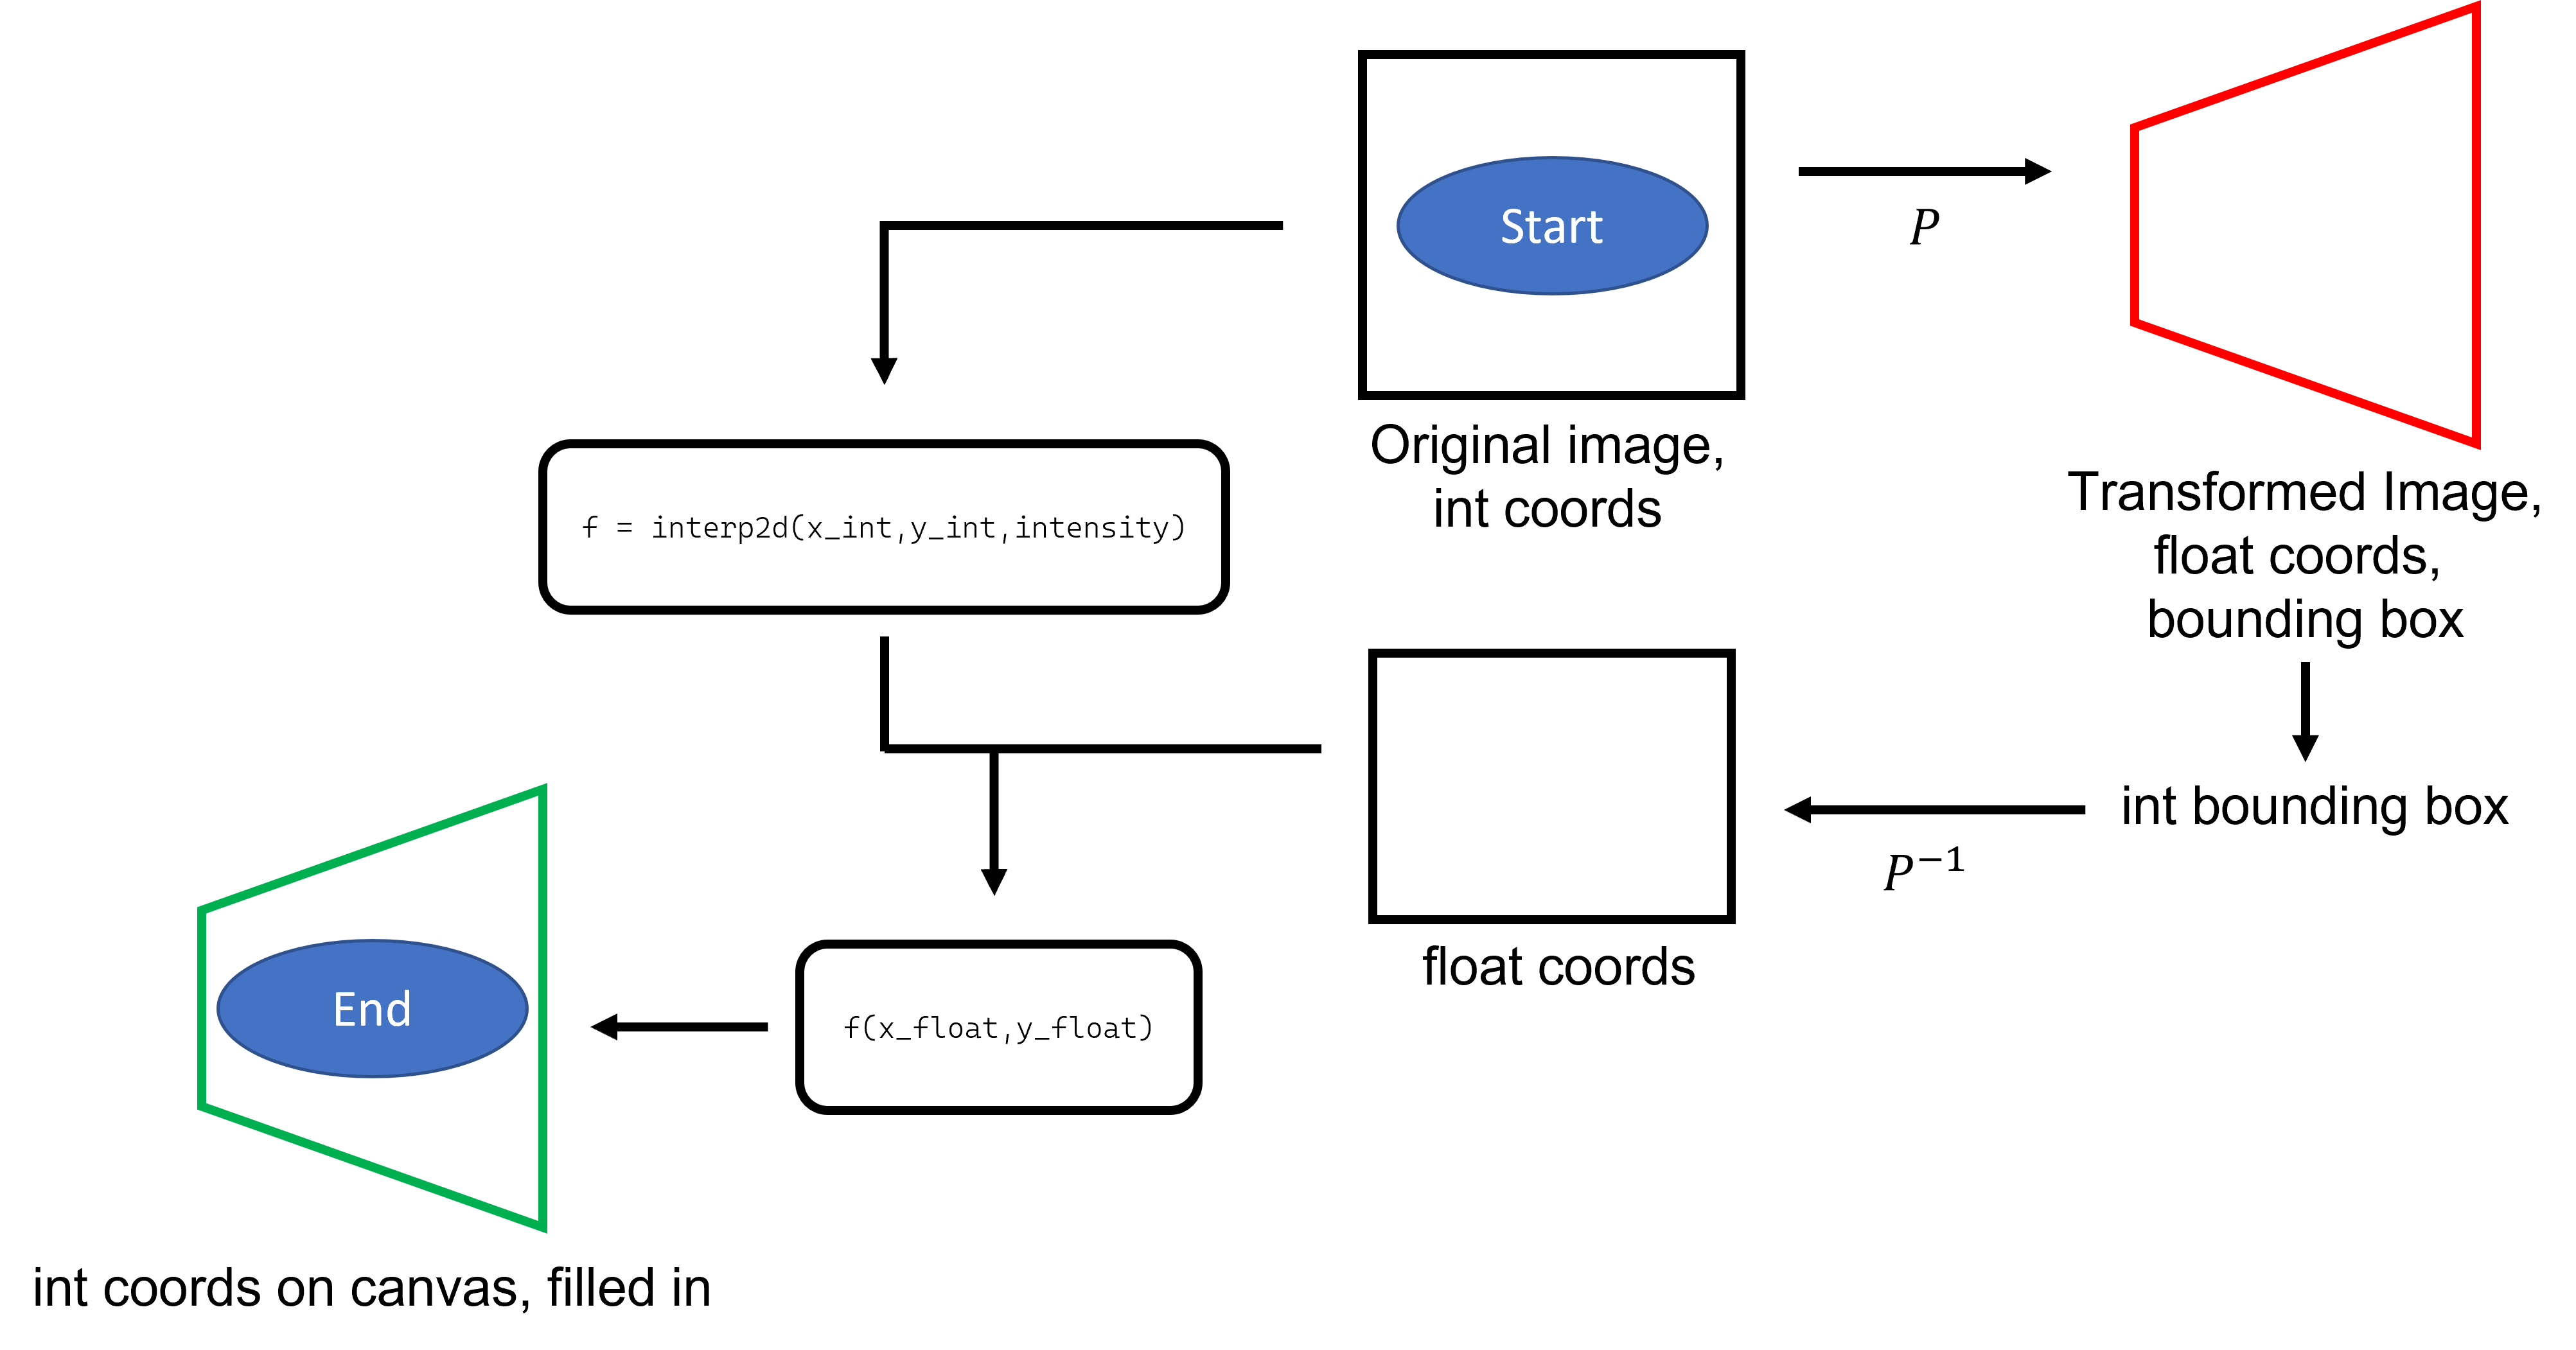
\includegraphics[width=6.5in]{test_images/interp_method.png}
	\caption{Proposed interpolation procedure.}
\end{figure}

\newpage

\section{Experiments}	
	\subsection{Given Dataset}
	I took the given images and formed the following mosaic with the procedure described above.
	
	\begin{figure}[H]
		\centering
		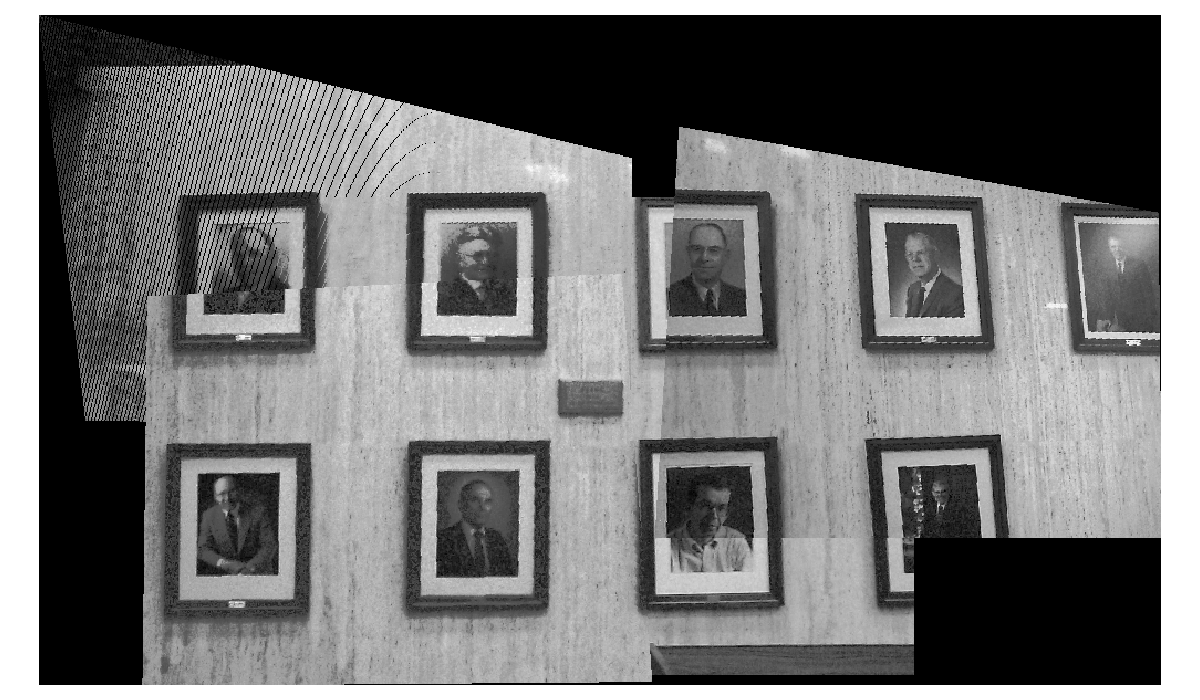
\includegraphics[width=6.5in]{test_images/hist_match.png}
		\caption{4 perspectively equivalent images made into a mosaic.}
	\end{figure}
	
	The large change in perspective of these images amplifies the black lines caused by the rounding method described above. These lines are most apparent in the upper left corner of the image.
	
	\newpage
	
	\subsection{Panoramic Images}
		I used the following panoramic images to see how the algorithm performs on them. This is using 10 correspondence points.
	\begin{figure}[H]
		\centering
		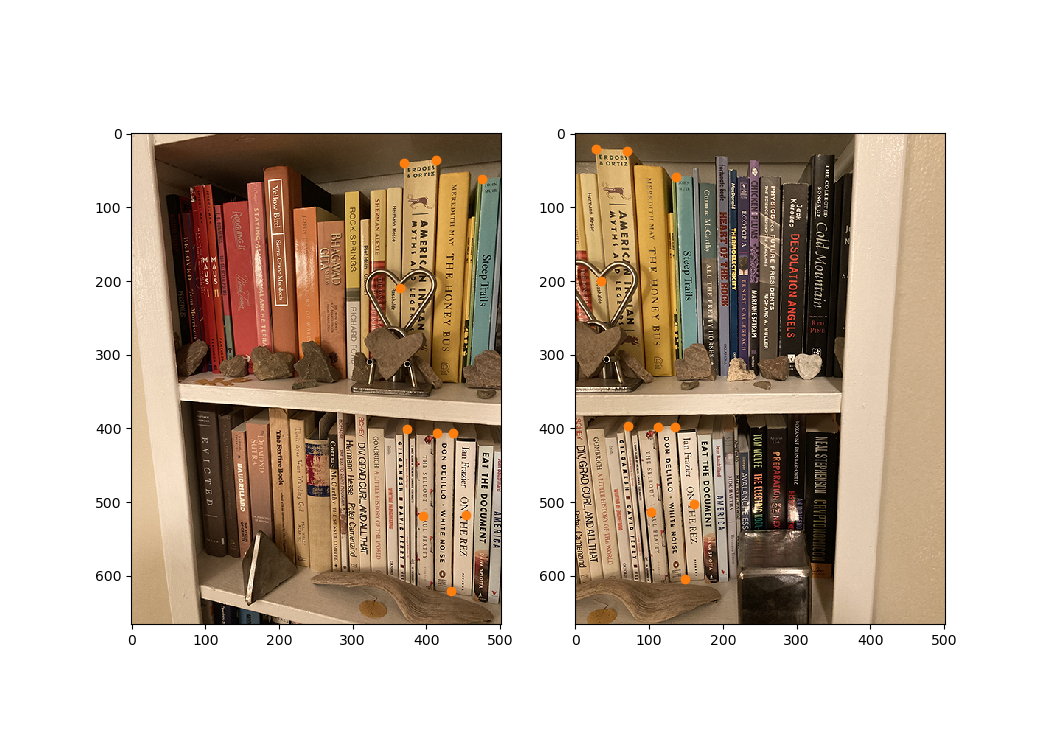
\includegraphics[width=6.5in]{test_images/shelf_10_correspondences.png}
		\caption{Bookshelf with 10 correspondences. I picked this image because it contains many corners, so accurately picking correspondences was straightforward.}
	\end{figure}

	\begin{figure}[H]
		\centering
		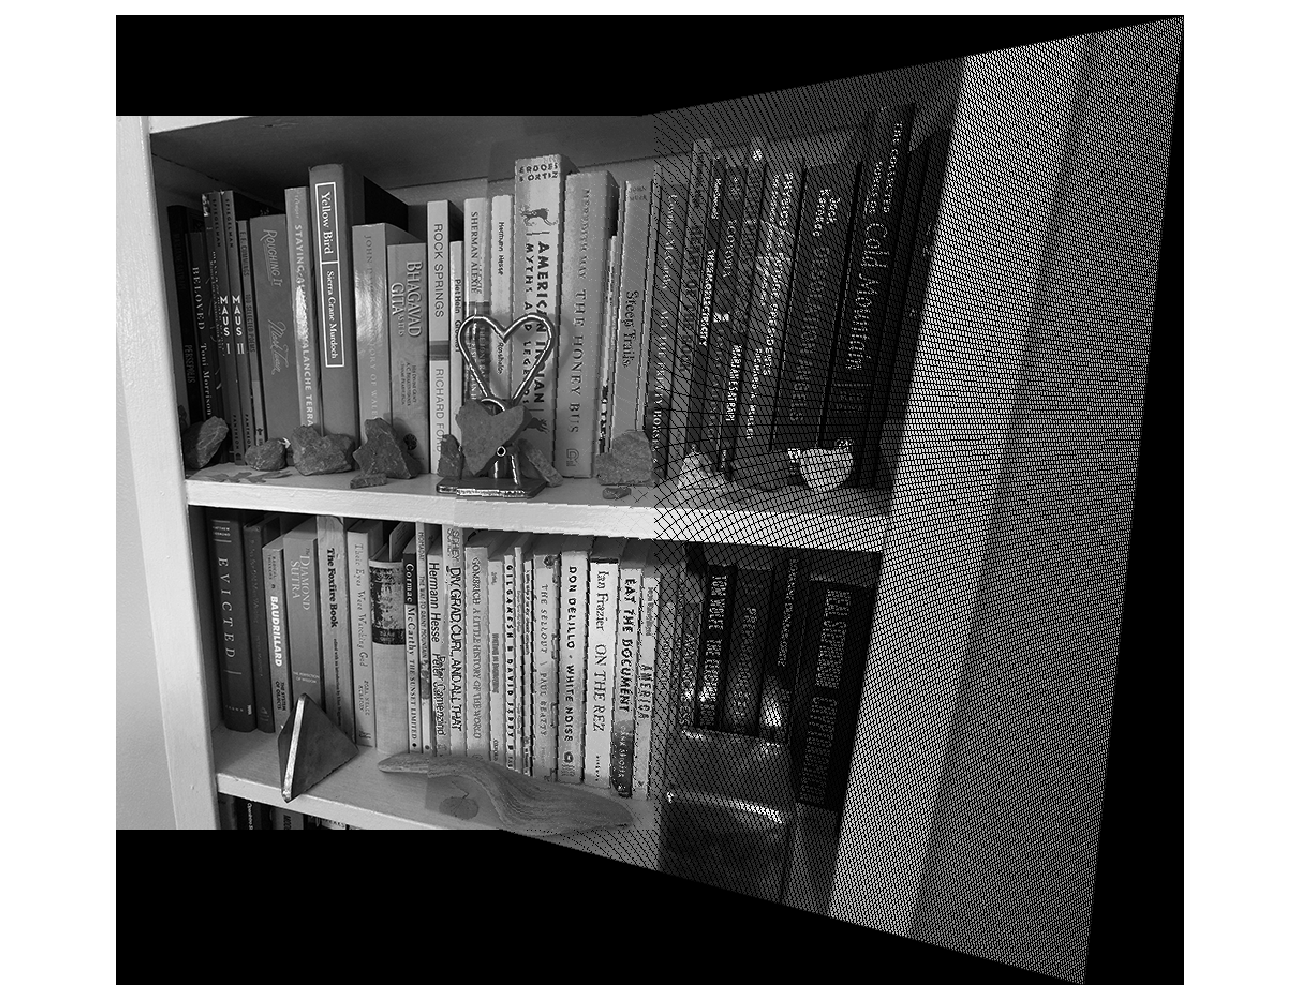
\includegraphics[width=6.5in]{test_images/shelf_10_floor.png}
		\caption{Mosaiced bookshelf with 10 correspondences. }
	\end{figure}

	Once again, the large perspective change amplifies the effect of the rounding method to introduce many warp contours. 

\newpage

	\subsection{Planar Images}
		I used the following planar images to see how the algorithm performs on them. Here I used 12 correspondence points, shown below.
		
		\begin{figure}[H]
			\centering
			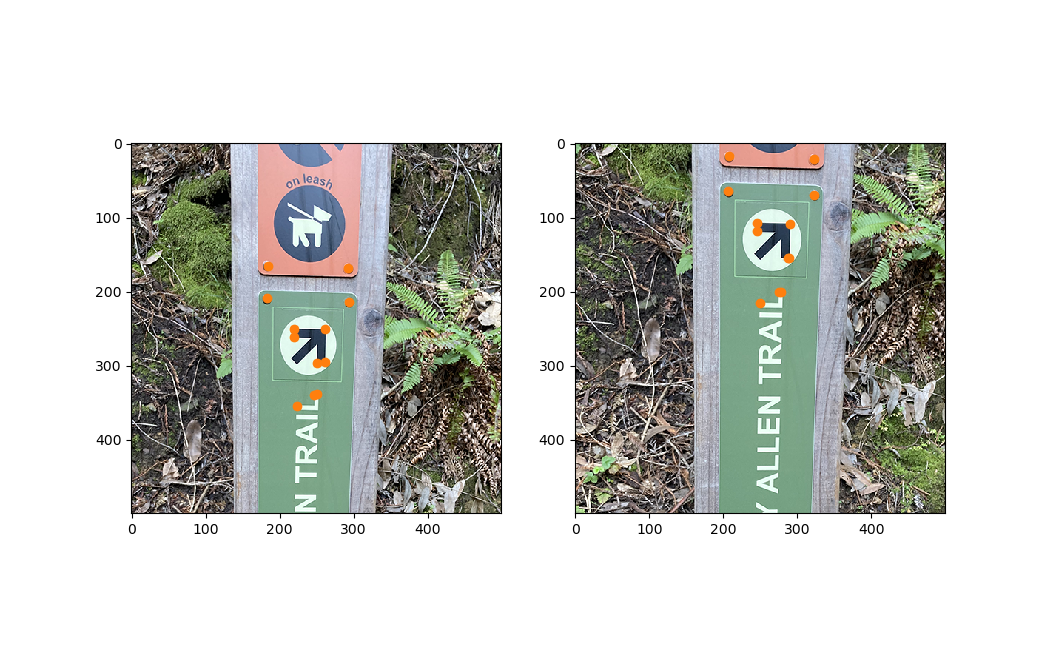
\includegraphics[width=6.5in]{test_images/sign_12_correspondences.png}
			\caption{Trail sign with 12 correspondences. I picked this image because it contains many corners, so accurately picking correspondences was straightforward.}
		\end{figure}
	
		\begin{figure}[H]
			\centering
			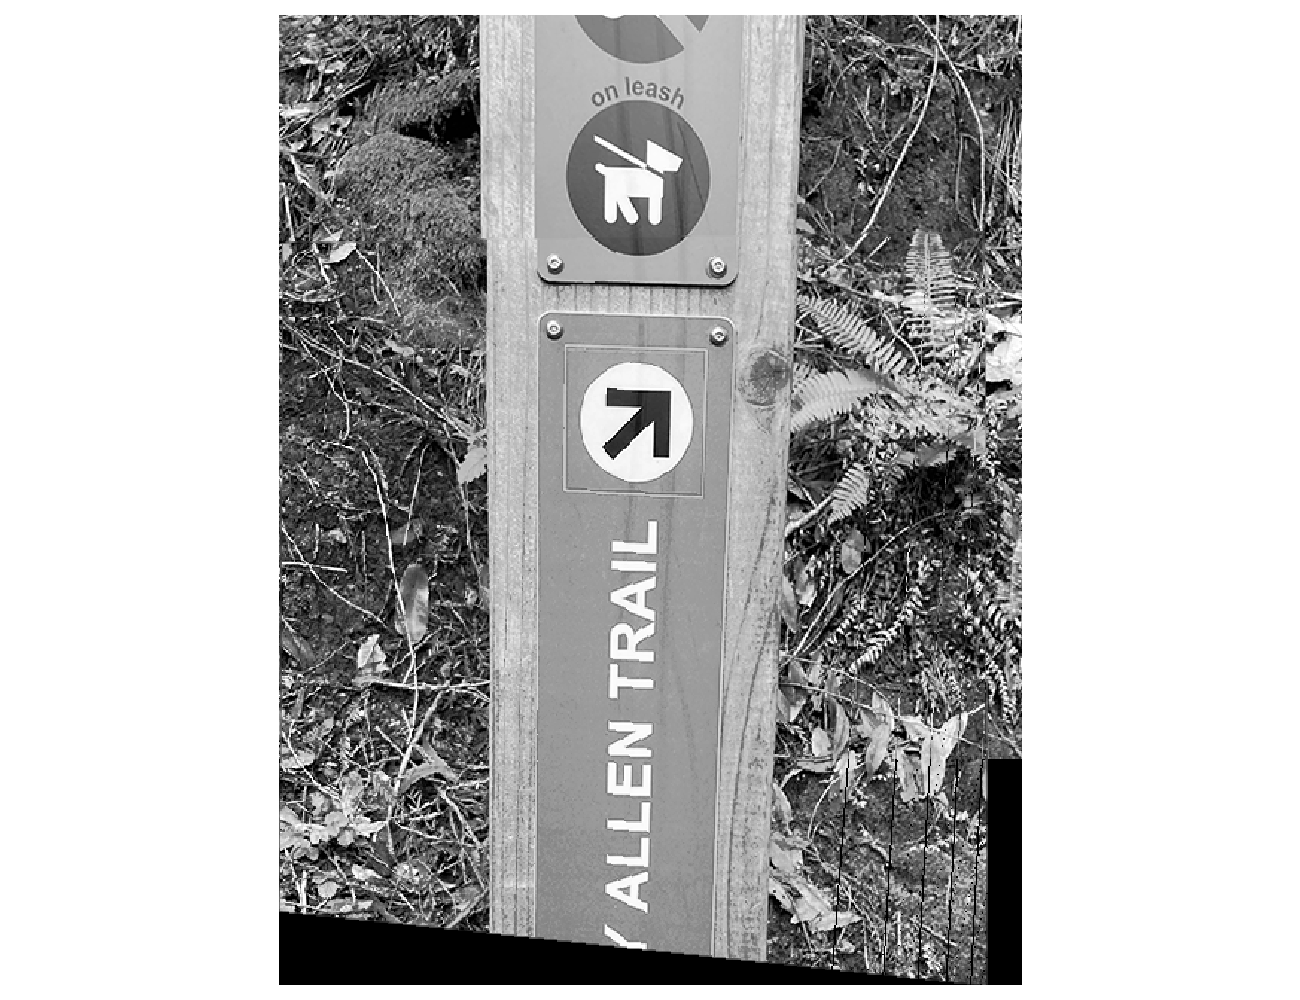
\includegraphics[width=6.5in]{test_images/sign_12_floor.png}
			\caption{Mosaiced trail sign with 12 correspondences. }
		\end{figure}
	Here, the minimal warping and minimal perspective change results in fewer contour lines and a less confusing image. 

	\newpage
		
	\subsection{Number of Correspondences}
	I experimented with the number of correspondence points on both the planar and panoramic images. 
	
	\subsubsection{Planar Images}
	\vskip 10pt
	I tried to use 4 correspondence points on the planar image shown above. I chose the number 4 because it is the theoretical minimum number of correspondence points needed to solve for the transformation. This worked with varying degrees of success. Some combinations of 4 of my total 12 correspondence points produced a mostly valid transformation, shown below. However some combinations of correspondence points did not work as well and would have produced a very large and ugly image. I attribute this to the correspondence points being chosen by hand, so they were not extremely accurate. 
	
	\begin{figure}[H]
		\centering
		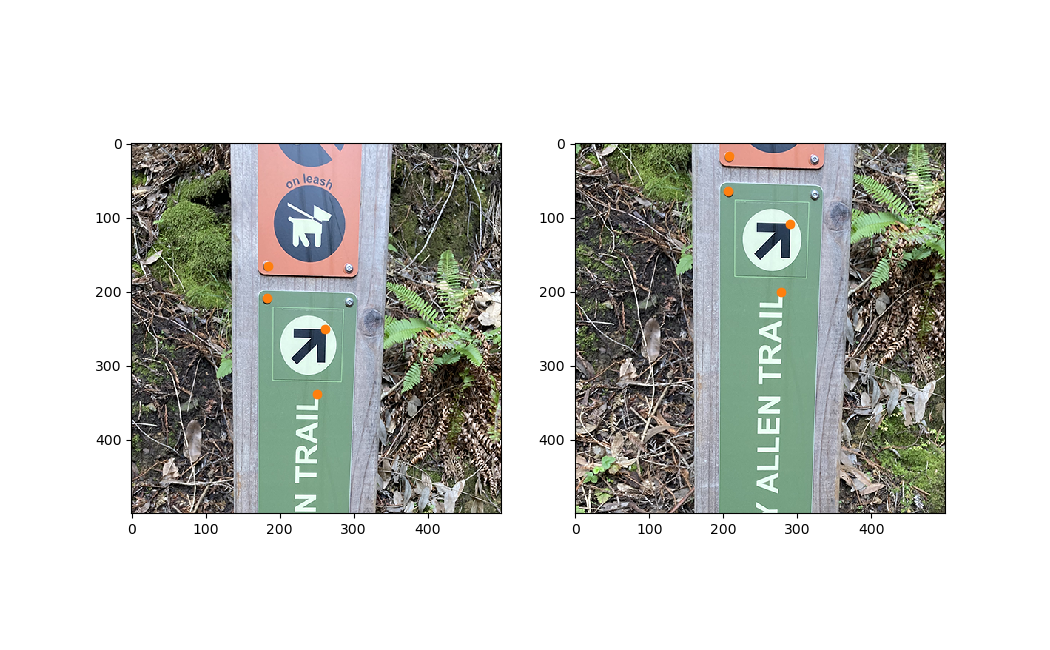
\includegraphics[width=6.5in]{test_images/sign_4_correspondences.png}
		\caption{Trail sign with 4 correspondences.}
	\end{figure}
	
	
	\begin{figure}[H]
		\centering
		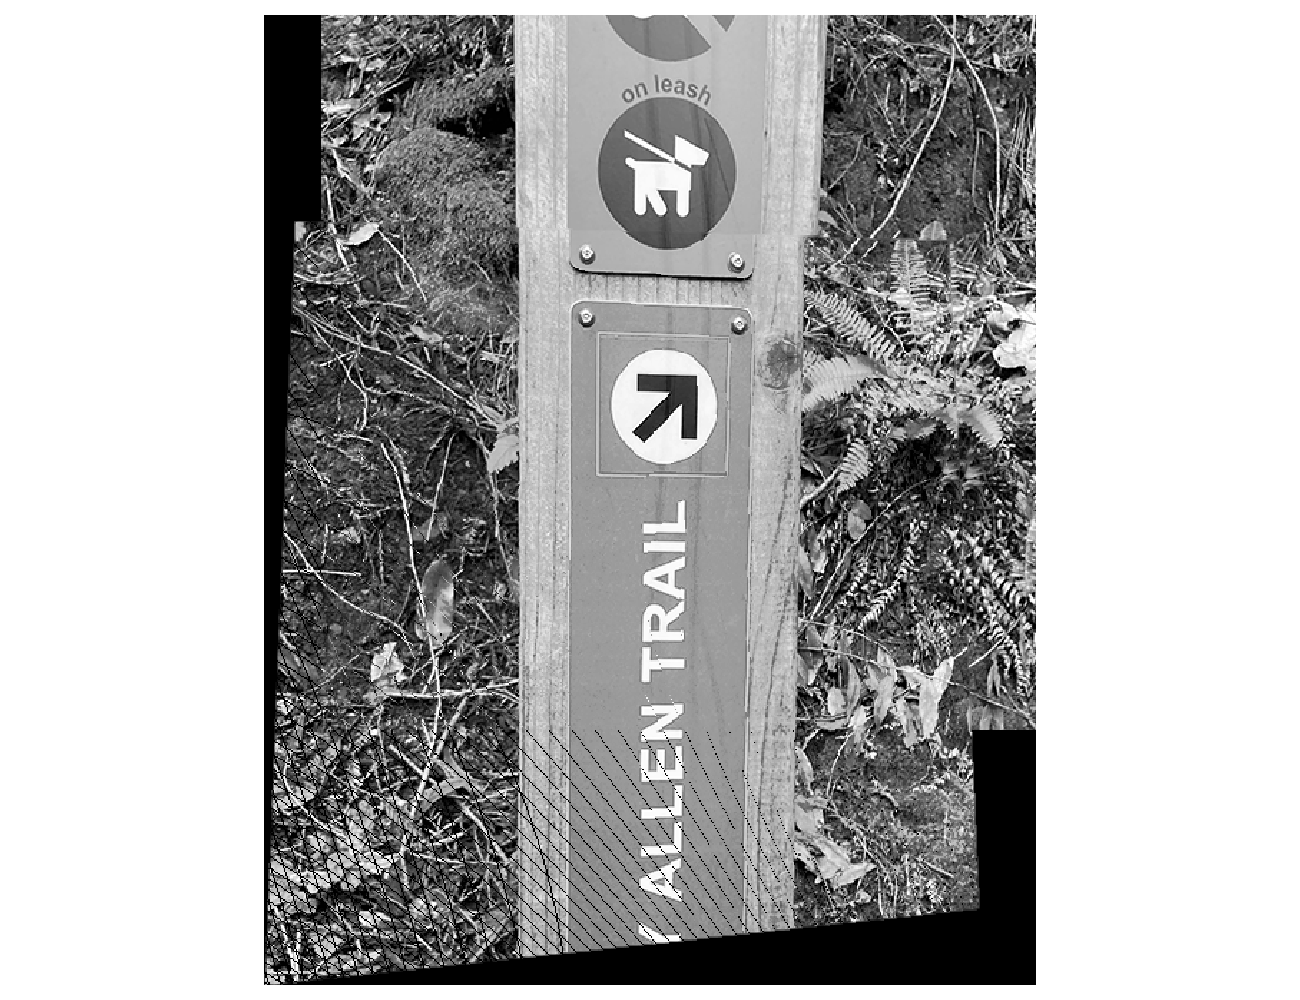
\includegraphics[width=6.5in]{test_images/sign_4_floor.png}
		\caption{Mosaiced trail sign with 4 correspondences. Things don't line up very well with so few correspondences. }
	\end{figure}

	\newpage
	
	Shown below again for clarity's sake is the same pair of images but constructed with a transformation informed by 12 correspondence points. This seemed to act as a filter on my imprecise correspondence point picking and generally make the image look better.
	
	\begin{figure}[H]
		\centering
		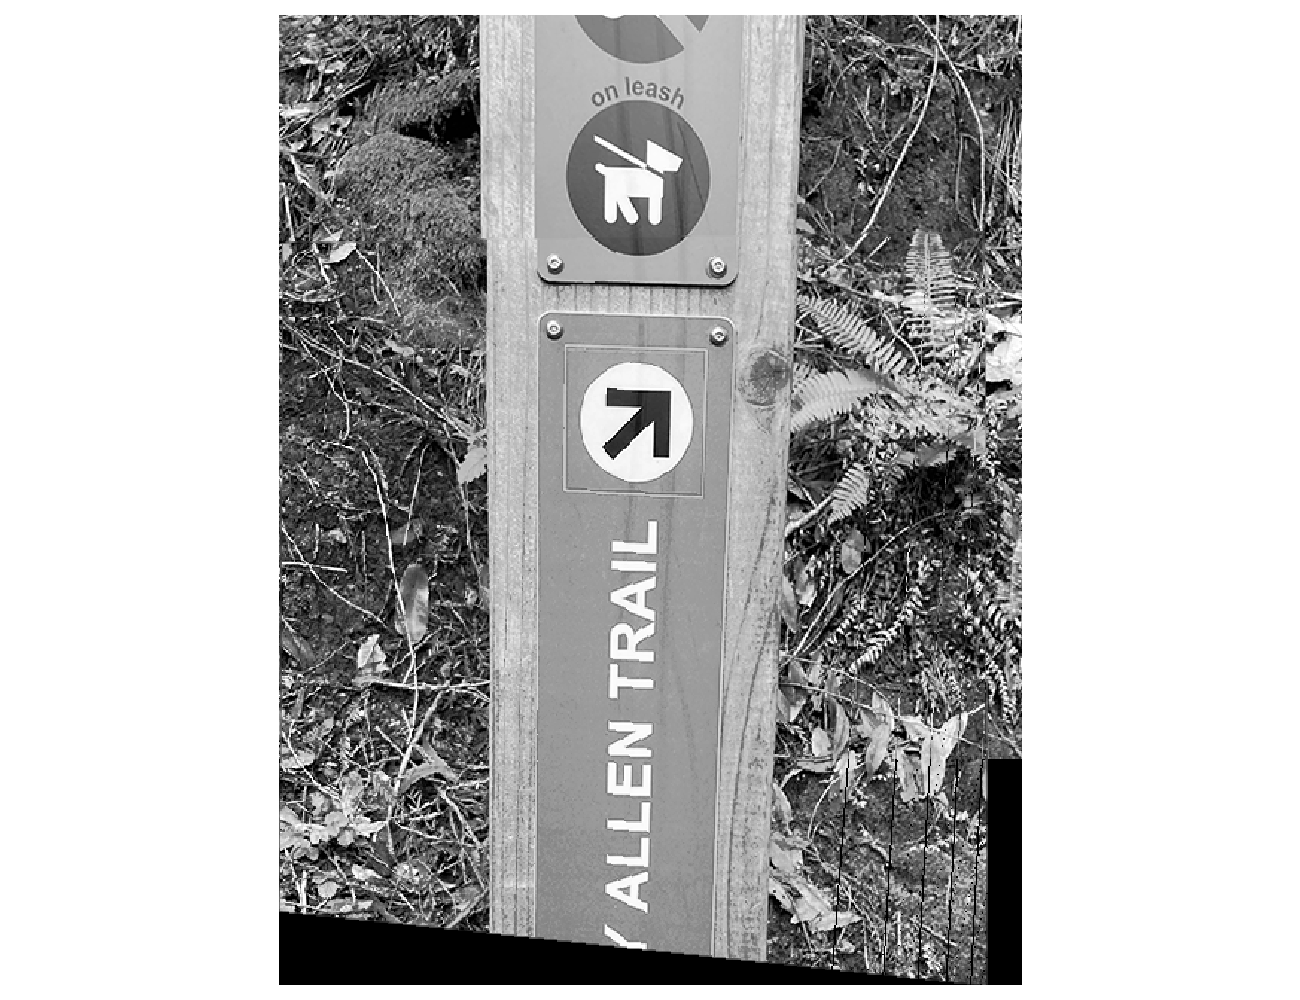
\includegraphics[width=6.5in]{test_images/sign_12_floor.png}
		\caption{Mosaiced trail sign with 12 correspondences. This lines up much better.}
	\end{figure}
	
	\newpage
	
	\subsubsection{Panoramic Images}
	I attempted to use 4 correspondence points on the panoramic images shown above, but I was unsuccessful. I encountered the same issue I described in the section on planar images where the transformation that was produced made too large of an image (orders of magnitude larger than the original images), so I added one correspondence point and successfully made a mosaic with 5 points. I attribute the lack of success to the large perspective change between the images. This is shown below.
	
	\begin{figure}[H]
		\centering
		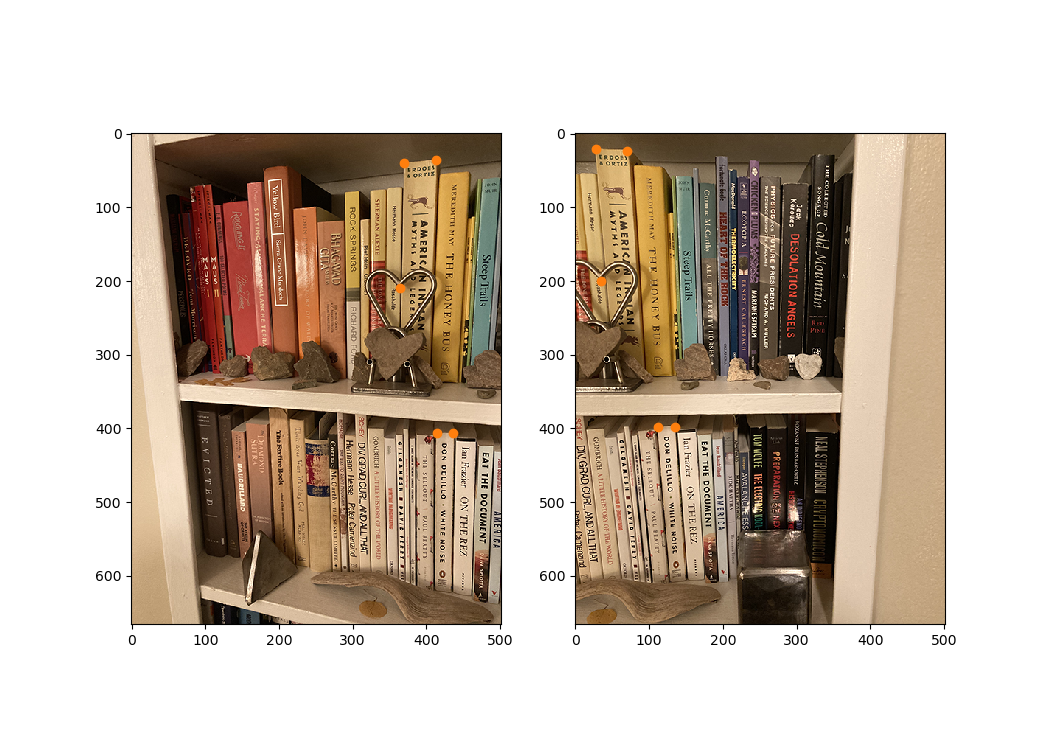
\includegraphics[width=6.5in]{test_images/shelf_5_correspondences.png}
		\caption{Bookshelf with 5 correspondences. I picked this image because it contains many corners, so accurately picking correspondences was straightforward.}
	\end{figure}
	
	\begin{figure}[H]
		\centering
		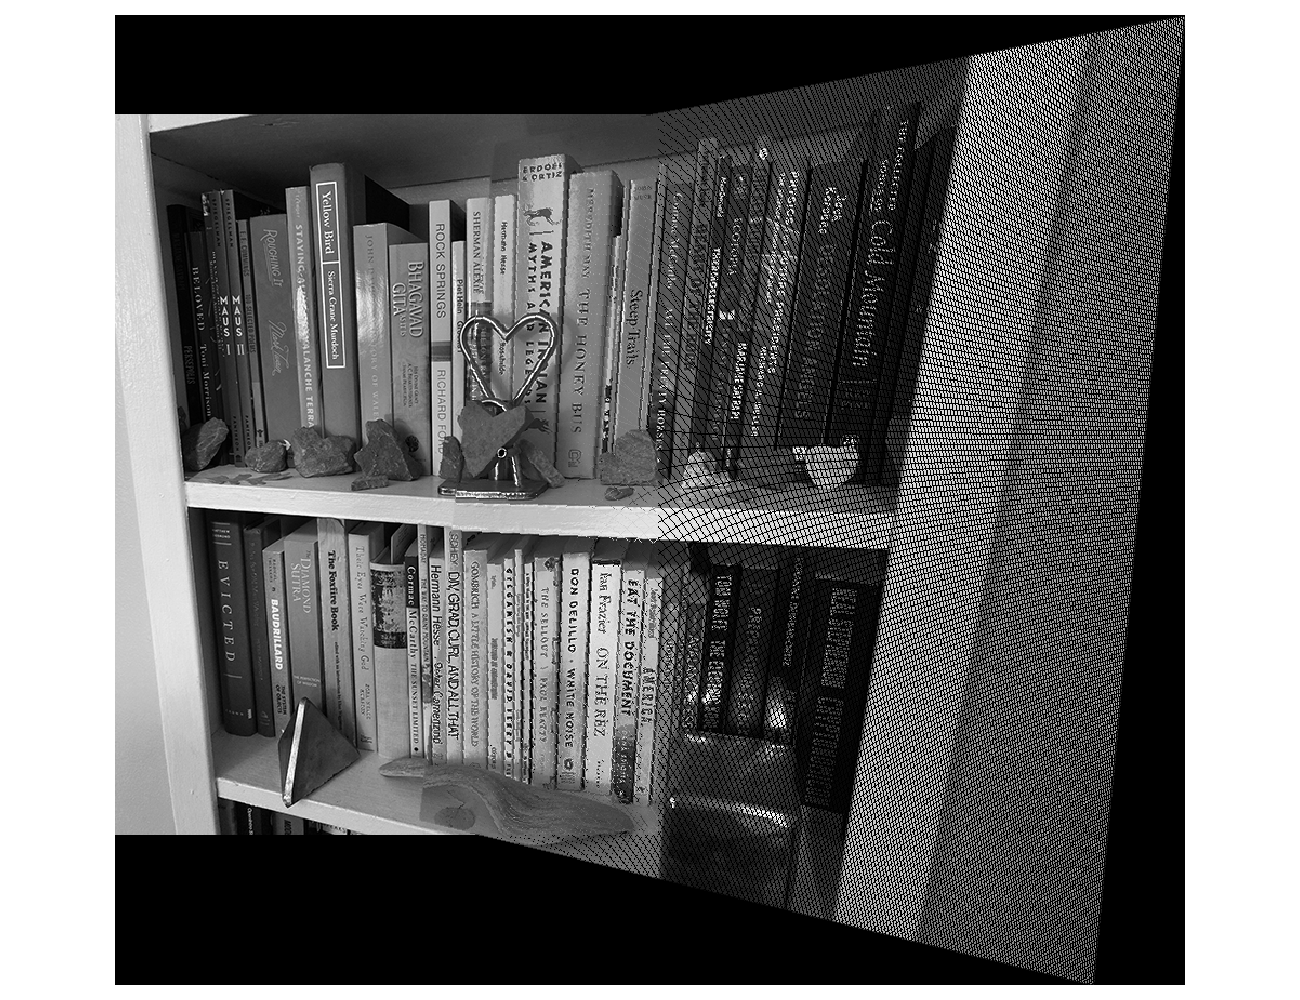
\includegraphics[width=6.5in]{test_images/shelf_5_floor.png}
		\caption{Mosaiced bookshelf with 5 correspondences. Notice the misalignment at the bottom left corner of the overlapping image.}	
	\end{figure}
	
	\newpage
	
	Shown again for clarity are the results from above with 10 correspondence points. In general, the image lines up slightly better, especially near the bottom.
	\begin{figure}[H]
		\centering
		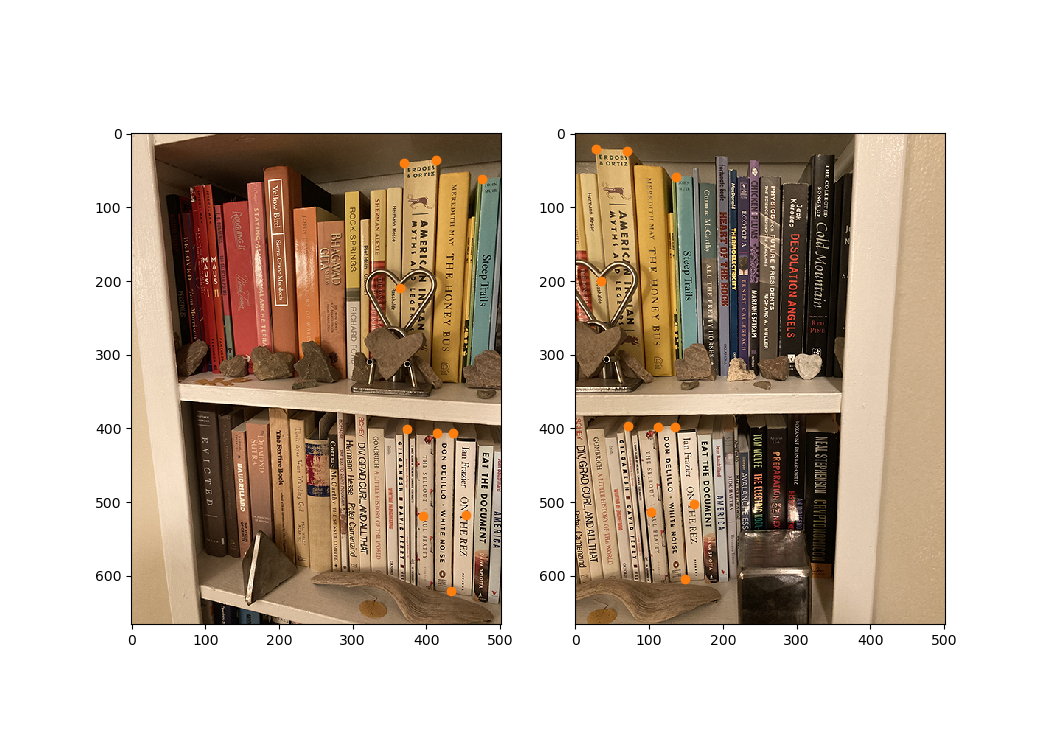
\includegraphics[width=6.5in]{test_images/shelf_10_correspondences.png}
		\caption{Bookshelf with 10 correspondences. }
	\end{figure}
	
	\begin{figure}[H]
		\centering
		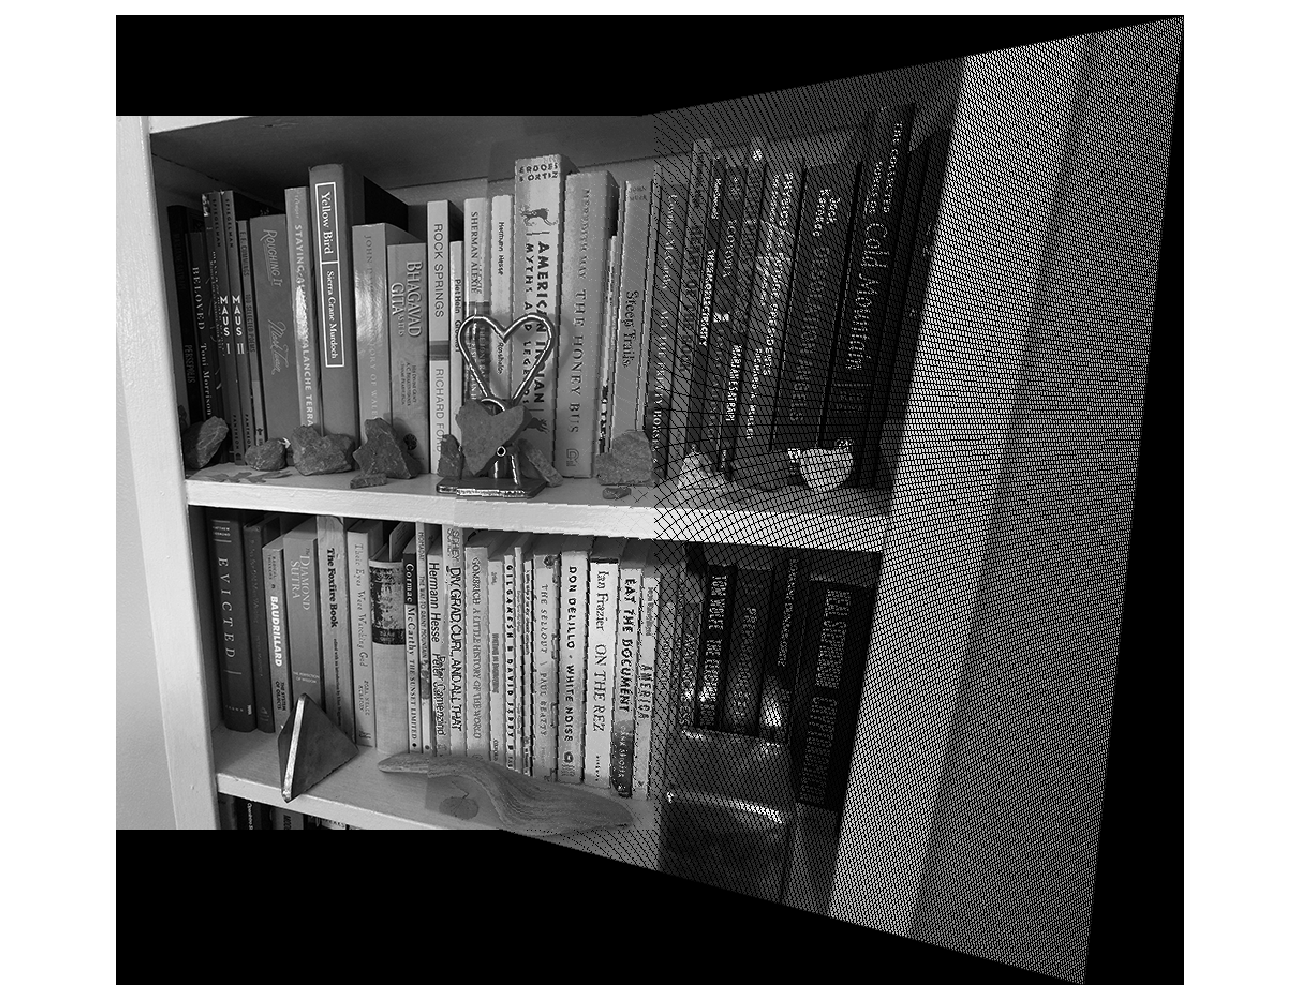
\includegraphics[width=6.5in]{test_images/shelf_10_floor.png}
		\caption{Mosaiced bookshelf with 10 correspondences. }
	\end{figure}

\newpage

\section{Questions}
	\subsection{How many control points does it take to get a `good' transformation between images?}
	My results in the preceding sections indicate that having more correspondence points results in a better image mosaic. Solving a system with SVD provides the least-squares solution, so this comports with our intuition regarding least-squares solutions and the central limit theorem, wherein the ``quality" or ``truth" of a prediction improves with the number of data points that are used to make it. From my own initial experimentation it seems that 8 or greater correspondence points capture enough of the truth of the perspective equivalence to construct a convincing image mosaic.
	
	\subsection{How does the algorithm behave at the theoretical minimum of the number of control points?}
		The theoretical minimum number of correspondence points is 4 because that is the minimum possible number of points that allows the matrix below to have full rank. If this matrix has at least rank 8 and the number of rows is equal to the rank, then the system has an analytical solution. If the system has at least rank 8 and the number of rows is greater than the rank, then the system has a least-squares solution.
		\[\left(\begin{array}{cccccccc}
			-x_{1} & -y_{1} & -1 & 0 & 0 & 0 & x_{1} x_{1}^{\prime} & y_{1} x_{1}^{\prime} \\
			-x_{2} & -y_{2} & -1 & 0 & 0 & 0 & x_{2} x_{2}^{\prime} & y_{2} x_{2}^{\prime} \\
			-x_{3} & -y_{3} & -1 & 0 & 0 & 0 & x_{3} x_{3}^{\prime} & y_{3} x_{3}^{\prime} \\
			-x_{4} & -y_{4} & -1 & 0 & 0 & 0 & x_{4} x_{4}^{\prime} & y_{4} x_{4}^{\prime} \\
			0 & 0 & 0 & -x_{1} & -y_{1} & -1 & x_{1} y_{1}^{\prime} & y_{1} y_{1}^{\prime} \\
			0 & 0 & 0 & -x_{2} & -y_{2} & -1 & x_{2} y_{2}^{\prime} & y_{2} y_{2}^{\prime} \\
			0 & 0 & 0 & -x_{3} & -y_{3} & -1 & x_{3} y_{3}^{\prime} & y_{3} y_{3}^{\prime} \\
			0 & 0 & 0 & -x_{4} & -y_{4} & -1 & x_{4} y_{4}^{\prime} & y_{4} y_{4}^{\prime}
		\end{array}\right)\left(\begin{array}{c}
			p_{11} \\
			p_{12} \\
			p_{13} \\
			p_{21} \\
			p_{23} \\
			p_{23} \\
			p_{31} \\
			p_{32}
		\end{array}\right)=\left(\begin{array}{c}
			-x_{1}^{\prime} \\
			-x_{2}^{\prime} \\
			-x_{3}^{\prime} \\
			-x_{4}^{\prime} \\
			-y_{1}^{\prime} \\
			-y_{2}^{\prime} \\
			-y_{3}^{\prime} \\
			-y_{4}^{\prime}
		\end{array}\right)\]
	
	The algorithm is temperamental when used with 4 correspondence points, and I attribute this to human error when picking correspondence points, as well as the inevitable lack of alignment/registration between the world frame and the camera frame. This means that physical objects in the world may get mapped to different fractions of pixels, and then as a result get rounded differently. The algorithm was particularly temperamental when I tried to use 4 correspondence points on the images of the bookshelf, so I ended up having a practical minimum number of 5 correspondence points. With just 4 points the transformation stretched out the second image to several orders of magnitude larger than it originally was, which was either unachievable with the current canvas size or indecipherable as an image with a canvas large enough to permit the image.
		
	\subsection{From your experiments, how does the accuracy of the control points affect the results?}
		To test this, I swapped two control points in one of the two images being mosaiced. I did this for an image that had 10 control points to begin with so that this experiment didn't completely derail the procedure. The results are shown below and they are wildly different from the results in the parts above. This indicates that the method is indeed sensitive to the accuracy of the control points, but not as bad as one might think. At first I only swapped one control point, but the results were not too bad. I imagine that this is due to the least-squares solution acting as a filter on outliers like this. 
		
		\begin{figure}[H]
			\centering
			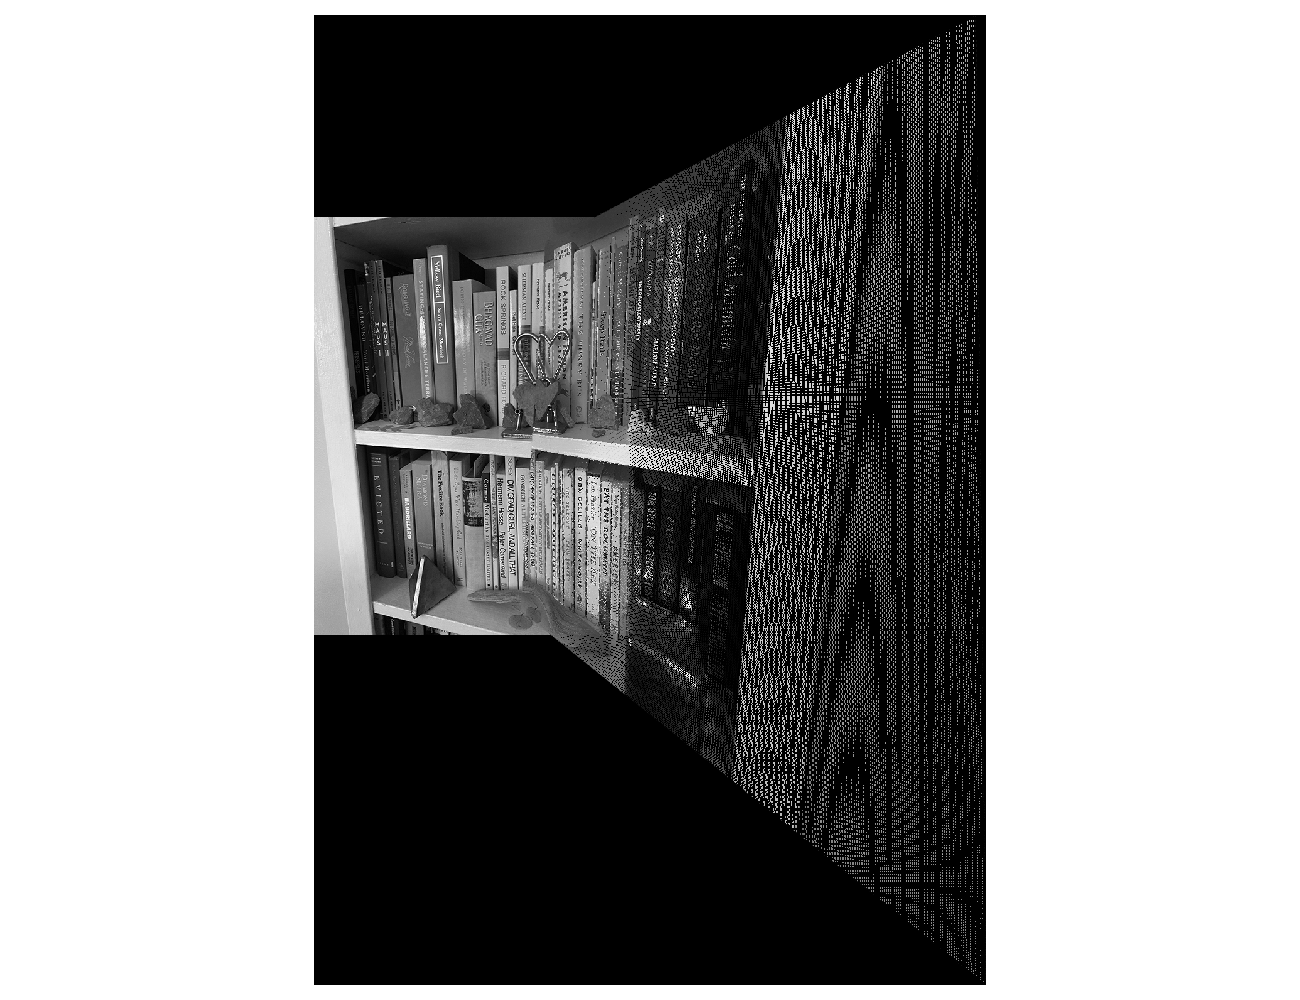
\includegraphics[width=6.5in]{test_images/shelf_10_mismatch.png}
			\caption{Mosaic with swapped control points. Swapping only two pairs of close-by points caused this effect.}
		\end{figure}

\section{Details}
	\subsection{Contrast}
	\label{contrast}
	\textbf{A good algorithm should automatically adjust for major intensity differences.}
	\vskip 10pt
	To handle this I used the \texttt{skimage.exposure.match\_histograms} function to match all of the histograms to the first image that I read in to the program. Below are some results with and without histogram matching. This seemed like the most logical way to solve this problem.
	
	\begin{figure}[H]
		\centering
		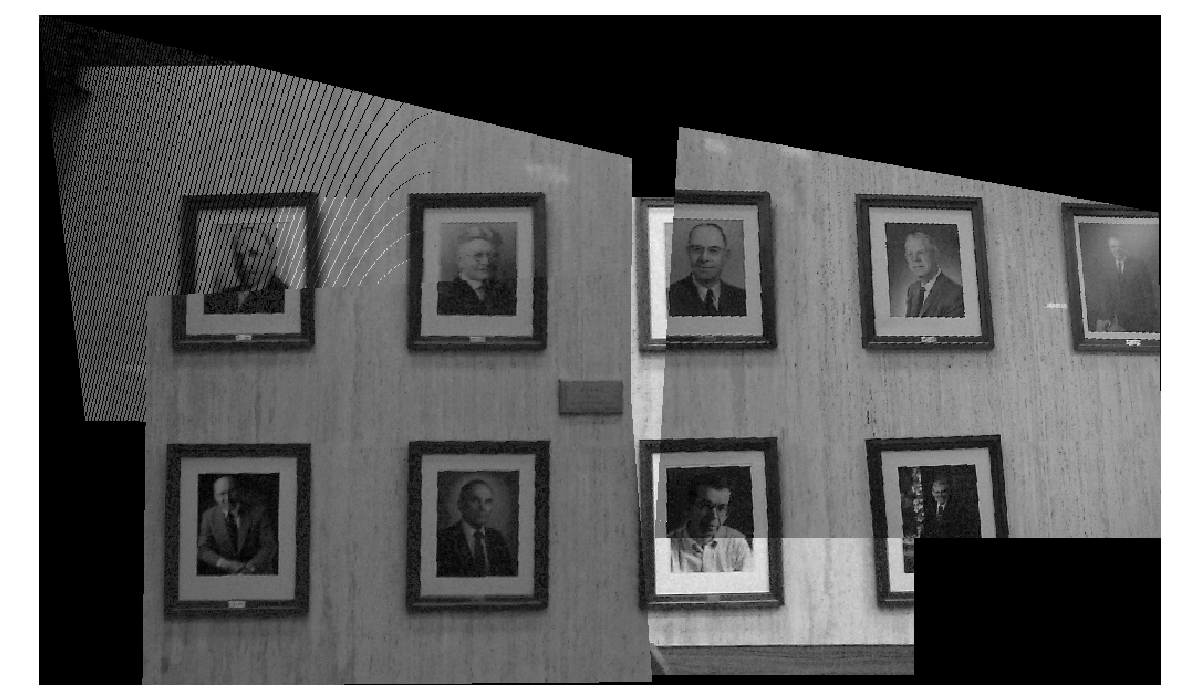
\includegraphics[width=6.5in]{test_images/no_hist_match.png}
		\caption{Mosaic with no histogram matching. Differences in intensity are very obvious and distracting.}
	\end{figure}
	
	\begin{figure}[H]
		\centering
		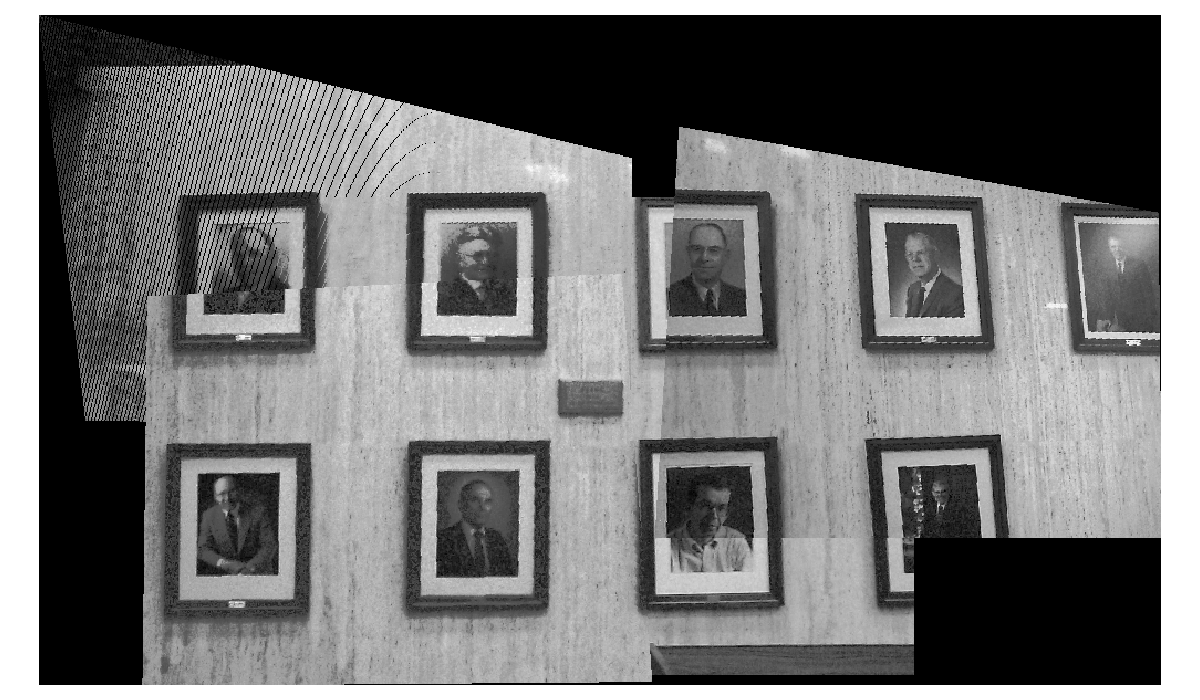
\includegraphics[width=6.5in]{test_images/hist_match.png}
		\caption{Mosaic with histogram matching. Differences in intensity are much less severe and are in general less distracting.}
	\end{figure}
	
	\subsection{Feathering}
	To blur the edges, I moved an averaging box filter around the edges of each warped image that I placed. The results are minimally effective but they are shown below. The code to execute this is located in the \texttt{feather()} function in the \texttt{functions.py} module included with this report. First, I show a representative path that the filter would move around to blur, then I show the image. Note that all of the images shown until this point have had their edges feathered with this method. 
	\begin{figure}[H]
		\centering
		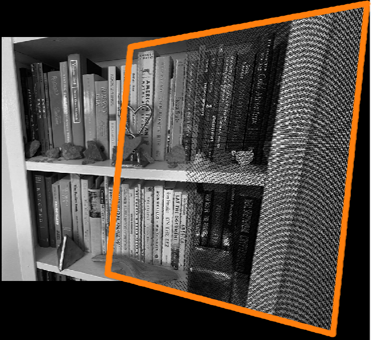
\includegraphics[width=4.5in]{test_images/shelf_10_orange.png}
		\caption{Representative path of an edge blending filter. This follows the perimeter of the overlaid image.}
	\end{figure}

	\begin{figure}[H]
		\centering
		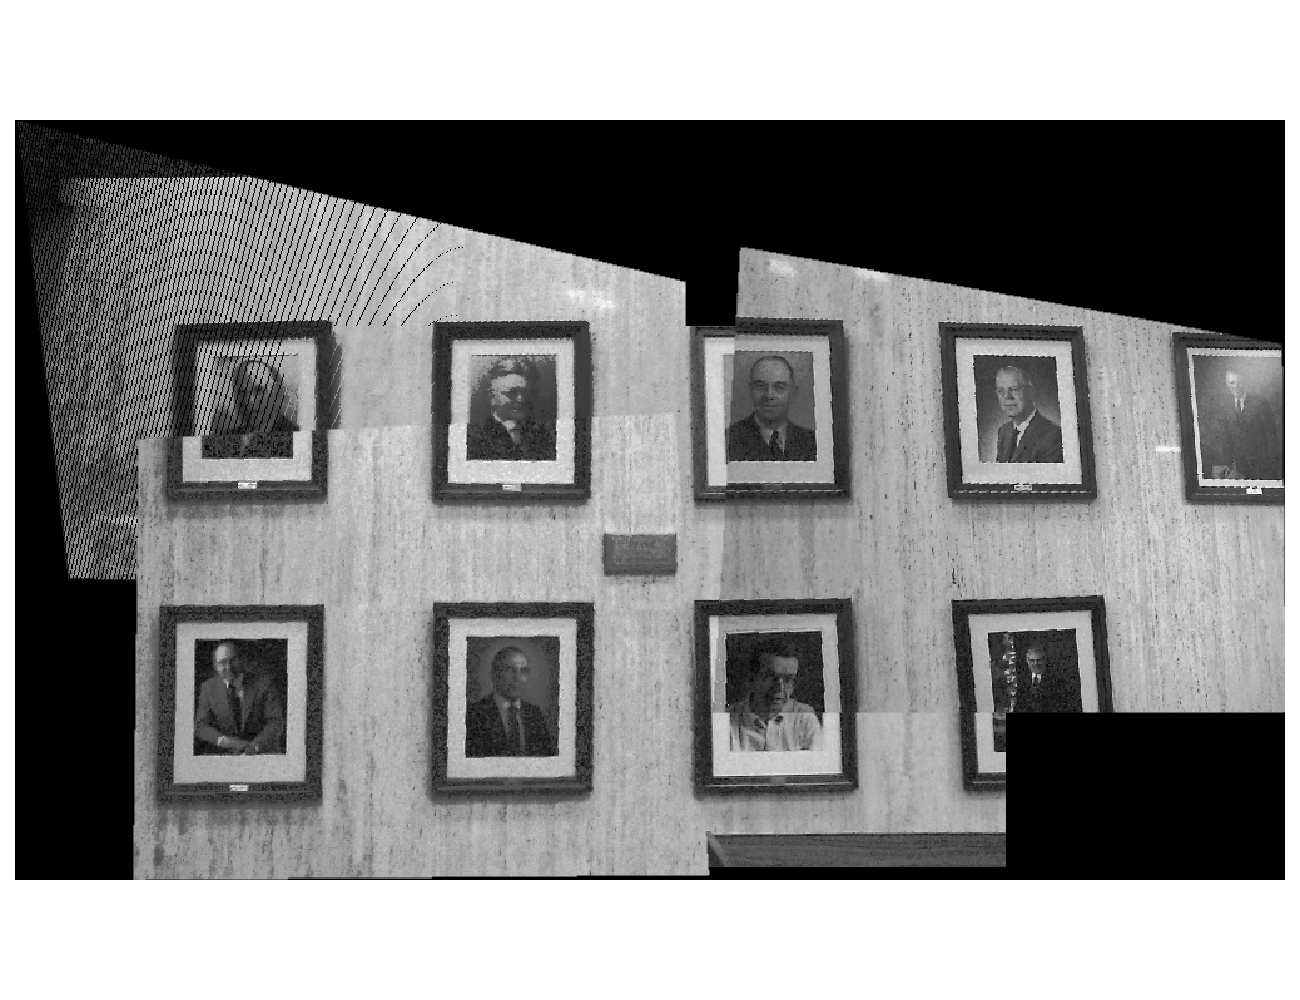
\includegraphics[width=6.5in]{test_images/example_raw.png}
		\caption{Edge blended mosaic. Results are minimally noticeable but add to the legibility.}
	\end{figure}
	
	
	
	\subsection{Image Size}
	Initially, for $n$ number of images, I make a canvas that is $n+1$ times the size of the largest image so that I have enough room to work with when placing images in the mosaic. However, this often results in a canvas which is much larger than it needs to be. To return the canvas to a more reasonable size for viewing once the mosaic is complete, I execute the following procedure. I search through the large canvas to find the first and last rows and columns which contain only zero elements. I do this by using the \texttt{numpy.sum()} function on each row and column and checking to see if it is equal to 0. The canvas consists of all zeros before I place images on it, so this method works by assuming that a row of all zeros contains no image information. I perform it this way because I figure that \texttt{numpy}'s vectorization is faster than my own implementation of computing the sum or individually inspecting every element in the image. This is implemented in the \texttt{trim\_canvas()} function in \texttt{functions.py}.
	
	\newpage
	
\section{Notes on Implementation}
	\begin{itemize}
	\item You must use my \texttt{read\_json.py} file.
	\item You must use my \texttt{mosaic\_params.json} file, and my other \texttt{.json} files provided with this report. 
	\item If you choose to use a separate \texttt{.json} file, ensure that the ordered pairs of the correspondences match the format in my images and parameter files.
	\item Ensure that there is a folder called \texttt{test\_images} in the directory that the python files are located.
	\item I have included a folder called \texttt{test\_images} in my submission in the correct location. It contains the base images I have used in this report. 
	
\end{itemize}



\end{document}          

